\section{Teleport Messaging}
\label{sec:teleport}

%% In this section we describe how $\sdep$ information can be
%% incorporated into the semantics of a language feature that provides
%% precise delivery of control messages in stream programs.  Our goal is
%% to improve performance as well as programmer productivity.\newline

Teleport messaging is a language construct that makes use of $\sdep$
to achieve precise timing of control messages.  It is included as part
of the StreamIt language~\cite{streamitcc}.  Teleport messaging
represents out-of-band communication between two actors, distinct from
the high-bandwidth dataflow in the stream graph.  Messages are
currently supported between any pair of actors with a meaningful
$\sdep$ relationship, i.e., wherever there is a directed path in the
stream graph from one actor to the other.  We say that a {\it
downstream} message travels in the same direction as the steady-state
data flow, whereas an {\it upstream} message travels against it.

\paragraph*{Syntax}  In order for actor $A$ to send a message to
actor $B$, the following steps need to be taken:
\begin{itemize}

\item $B$ declares a message handler that is invoked when a
message arrives.  For example: {
\vspace{-5pt}
\begin{verbatim}
handler increaseGain(float amount) {
  this.gain += amount;
}
\end{verbatim}
\vspace{-5pt}}
Message handlers are akin to normal functions, except that they
cannot access the input/output channels and they do not return values.

For another example, see line 40 of Figure~\ref{fig:fir-message-code}.

\item A parent stream containing $A$ and $B$ declares a variable of
type {\tt portal<}$T_B$\hspace{-1pt}{\tt >} that can forward messages
to one or more actors of type $T_B$.  The parent adds $B$ to the
portal and passes the portal to $A$ during initialization.

For example, see lines 8, 10 and 12 of Figure~\ref{fig:fir-message-code}.

\item To send a message, $A$ invokes the handler method on the portal
from within its steady-state work function. The handler invocation
includes a range of latencies {\tt [min:max]} specifying when the
message should be delivered; if no latency is specified, then a
default latency of {\tt [0:0]} is used.  The following illustrates an
example.{
\vspace{-12pt}
\begin{verbatim}
work pop 1 {
  float val = pop();
  if (val < THRESHOLD) {
    portalToB.increaseGain(0.1) [2:3];
  }
}
\end{verbatim}\vspace{-5pt}}
This code sends an {\tt increaseGain} message to {\tt portalToB} with
minimum latency 2 and maximum latency 3.

For another example, see line 25 of Figure~\ref{fig:fir-message-code}.
\end{itemize}
\paragraph*{Informal Semantics} The most interesting aspect of teleport
messaging is the semantics for the message latency.  Because there
are many legal orderings of actor executions, there does not exist a
notion of ``global time'' in a stream graph.  The only common frame of
reference between concurrently executing actors is the series of data
items that is passed between them.

Intuitively, the message semantics can be thought of in terms of
attaching tags to data items.  If $A$ sends a message to downstream
actor $B$ with a latency $k$, then this could be implemented by
tagging the items that $A$ outputs $k$ iterations later.  These tags
propagate through the stream graph; whenever an actor inputs an item
that is tagged, all of its subsequent outputs are tagged.  Then, the
message handler of $B$ is invoked immediately before the first
invocation of $B$ that inputs a tagged item.  In this sense, the
message has the semantics of traveling ``with the data'' through the
stream graph, even though it is not necessarily implemented this way.

The intuition for upstream messages is similar.  Consider that $B$ is
sending a message with latency $k$ to upstream actor $A$ in the stream
graph.  This means that $A$ will receive the message immediately
after its last invocation that produces an item affecting the output
of $B$'s $k$th firing, counting the current firing as 0.  As before,
we can also think of this in terms of $A$ tagging items and $B$
observing the tags.  In this case, the latency constraint says that
$B$ must input a tagged item before it finishes $k$ additional
executions.  The message is delivered immediately after the latest
firing in $A$ during which tagging could start without violating this
constraint.

\paragraph*{Formal Semantics} The $\sdep$ function captures the
data dependences in the graph and provides a natural means of defining
a rendezvous point between two actors.  The following definition
leverages $\sdep$ to give a precise meaning to message timing.

\begin{definition}(Message delivery)
Consider that $S$ sends a message to receiver $R$ with latency range
$[k_1:k_2]$ and that the message is sent during the $n$th execution of
$S$.  There are two cases\footnote{\small In a feedback path, both
cases might apply.  In this event, we assume the message is being sent
upstream.}:

\begin{enumerate}

\item If $R$ is downstream of $S$, then the message handler must be
invoked in $R$ immediately before its $m$th execution, where $m$
is constrained as follows:
\[
\begin{array}{l}
n+k_1 \le \sdepf{S}{R}(m) \le n+k_2
%\sdepf{S}{R}(m) \ge n+k_1\\
%\sdepf{S}{R}(m) \le n+k_2
\end{array}
\]

\item If $R$ is upstream of $S$, then the message handler must be
invoked in $R$ immediately after its $m$th execution, where $m$ is
constrained as follows:
\[
\begin{array}{l}
%m \ge \sdepf{R}{S}(n + k_1)\\
%m \le \sdepf{R}{S}(n + k_2)
\sdepf{R}{S}(n + k_1) \le m \le \sdepf{R}{S}(n + k_2)
\end{array}
\]
\end{enumerate}
\end{definition}

For example, consider the FIR code in
Figure~\ref{fig:fir-message-code}.  On line 25, the {\tt Source} sends
a message to the {\tt Multiply} actors with zero latency ($k_1 = k_2 =
0$).  Consider that, as illustrated in
Figure~\ref{fig:fir-message-diagram}, a message is sent during the
fifth execution of {\tt Source} ($n = 5$).  Because each {\tt
Multiply} is downstream of {\tt Source}, the following equation
constrains the iteration $m$ at which the message should be delivered
to a given {\tt Multiply}:
\begin{equation*}
\begin{array}{c}
n+k_1 \le \sdepf{Source}{Multiply}(m) \le n + k_2 \\[0.9Ex]
5 \le \sdepf{Source}{Multiply}(m) \le 5 \\[0.9Ex]
5 \le m \le 5 \\[0.9Ex]
m = 5
\end{array}
\end{equation*}
To calculate $\sdepf{Source}{Multiply}$, observe that {\tt Source}
produces one item per iteration, while each {\tt Multiply} produces
one item and consumes one item.  Thus, the {\tt Source} must fire $m$
times before any given {\tt Multiply} can execute $m$ times, and
$\sdepf{Source}{Multiply}(m) = m$.  Substituting into the above
equation yields $m=5$.  That is, the message is delivered to each {\tt
Multiply} immediately before its fifth execution.  This is illustrated
in Figures~\ref{fig:fir-message-diagram}(c)
and~\ref{fig:fir-message-diagram}(d) for the first and second {\tt
Multiply} in the pipeline, respectively.  The message arrives
immediately before the fifth data item (which corresponds to the fifth
execution).

\paragraph*{Constraints on the Schedule}  
\label{sec:constraints}
It is important to recognize that messaging can place constraints on
the execution schedule.  The different categories of constraints are
illustrated in Figure~\ref{tab:messcons}.  A negative-latency
downstream message has the effect of synchronizing the arrival of the
message with some data that was previously output by the sender (e.g.,
for the checksum example mentioned in the introduction).  The latency
requires the downstream receiver not to execute too far ahead (i.e.,
too close to the sender), or else it might process the data before the
message arrives.  This translates to a constraint on the minimum
allowable latency between the sender and receiver actors in the
schedule for the program.  Intuitively, it also constrains the
buffering of data: the data buffers must not grow too small, as
otherwise the receiver would be too far ahead.

Similarly, a non-negative-latency upstream message places a constraint
on the maximum allowable latency between the sender and receiver.
This time the upstream actor must be throttled so that it does not get
too far ahead before the message arrives.  Intuitively, the amount of
data buffered between the actors must not grow too large.

\begin{figure}[t]
\begin{center}
\vspace{4pt}
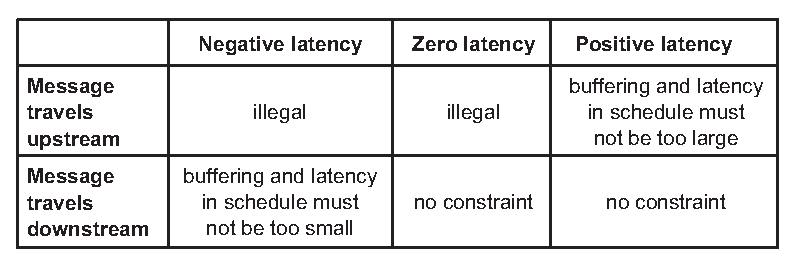
\psfig{file=constraints.eps,width=3in}
\vspace{-4pt}
\caption{\small Scheduling constraints imposed by messages.}
%% {\small
%% \begin{tabular}{|r|c|c|} \hline
%% ~ & {\bf Negative latency} & {\bf Positive latency} \\ \hline
%% {\bf Message travels downstream} & buffering and latency in schedule must not be too small & no constraint \\ \hline
%% {\bf Message travels upstream} & illegal & buffering and latency in schedule must not be too big \\ \hline
%% \end{tabular}}
\label{tab:messcons}
\end{center}
\vspace{-18pt}
\end{figure}

For upstream messages with negative latency, there always exist
iterations of the sender during which any messages sent are
impossible to deliver.  Consider an iteration of the sender that is
the first to depend on data propagating from the $n$th execution of
the receiver.  A negative-latency message would be delivered
immediately after a {\it previous} iteration of the receiver, but
since iteration $n$ has already fired, the message is impossible to
deliver.  Conversely, a downstream message with positive or zero
latency imposes no constraint on the schedule, as the sender has not
yet produced the data that is synchronized with the message.

\paragraph*{Unsatisfiable Constraints}  
Messaging constraints can be unsatisfiable---that is, assuming a
message is sent on every iteration of the sender's work function,
there does not exist a schedule that delivers all of the messages
within the desired latency range.  Such constraints should result in a
compile-time error.  

Figure~\ref{fig:infeasible} illustrates an example of unsatisfiable
constraints.  Though each messaging constraint is feasible in
isolation, the set of constraints together is unsatisfiable.  The
unsatisfiability is caused by conflicting demands on the buffering
between B and C.  The message from B to C constrains this buffer to
contain at least 10 items, while the message from D to A constrains it
to be empty.  We say that these two constraints {\it overlap} because
the paths from sender to receiver intersect a common actor in the
stream graph.
\begin{figure}[t]
\begin{center}
\psfig{figure=infeasible-messaging.eps,height=1.43in}
\vspace{-8pt}
\caption{{\small Example of unsatisfiable message constraints.  Each
node is annotated with its input and output rate.  Messages are shown
by dotted arrows, drawn from sender to receiver with a given latency.
The constraints are satisfiable in isolation, but unsatisfiable in
combination.  \protect\label{fig:infeasible}}}
\end{center}
\vspace{-13pt}
\end{figure}

\paragraph*{Finding a Schedule}
In the presence of overlapping constraints, we leave to future work
the problem of finding a legal execution schedule (if one exists).
Because overlapping constraints can be detected statically, a given
compiler may choose to prohibit overlapping constraints altogether.
%A discussion of the issues involved appears in a
%thesis~\cite{karczma-thesis} by one of the authors.

\begin{figure}[t]
\vspace{-12pt}
\psfig{figure=fhr-streamit.eps,width=3.35in}
\vspace{-20pt}
\caption{\small Stream graph of frequency hopping radio with teleport messaging.  
A portal delivers point-to-point latency-constrained messages from the
detectors to the RFtoIF stage.
\protect\label{fig:fhr-streamit}}
\vspace{-12pt}
\end{figure}

\begin{figure}[t]
\vspace{-12pt}
\hspace{-0.2in}\psfig{figure=code-freq1.eps,width=3.5in}
\vspace{-24pt}
\caption{\small Frequency hopping radio with teleport messaging.
Arrows depict the path of messages from the sender to the receiver,
via a portal declared in the top-level stream.
\protect\label{fig:freq1}}
\vspace{-12pt}
\end{figure}


For the case of non-overlapping constraints, a simple modification to
pull scheduling will always result in a legal schedule (if one
exists).  First, note that a pull schedule always satisfies
constraints imposed by upstream messages; because upstream (receiving)
actors execute as little as possible per execution of the downstream
(sending) actor, a message can be forwarded to the receiver
immediately after sending.  The receiver can then store the message
and process it at the appropriate iteration.  For downstream messages,
the pull scheduler is modified to always execute one iteration of the
upstream (sending) actor before any execution of the downstream
(receiving) actor that would exceed the latency range.  If the
upstream actor needs more inputs to fire, then they can always be
generated by actors that are further upstream (via a recursive call to
the pull scheduling algorithm).

As described in Section~\ref{sec:evaluation}, our compiler uses a
simple implementation of messaging in which each sender or receiver
executes in its own thread and waits for possible messages at
appropriate iterations.  This approach does not depend on producing a
serial ordering of the actors at compile time.

%\begin{figure}[t]
\begin{center}
\psfig{figure=constrained-example.eps,height=1.5in}
\caption{{\small Example of construction of a constrained schedule. The $\sdepf{R}{S}$ function for filters $R$ and $S$ is given in Table \ref{tab:sdepconst}. The blob between filters $R$ and $S$ illustrates other possible stream elements. $R$ sends a message to $S$ with latency $[1,2]$. Executions of the blob are ommitted, it is assumed that at the point $S$ executes, the blob has drained data provided by $R$.}}
\end{center}
\vspace{-12pt}
\label{fig:sdepconst}
\end{figure}

\begin{table*}[t]
{\small
\begin{tabular}{|c|c|} \hline
{\bf $sdepf{R}{S}$} & {\bf Execs of S} \\ \hline
$9n+2$ & $8n+1$ \\ \hline
$9n+3$ & $8n+2$ \\ \hline
$9n+5$ & $8n+3$ \\ \hline
$9n+5$ & $8n+4$ \\ \hline
$9n+6$ & $8n+5$ \\ \hline
$9n+8$ & $8n+6$ \\ \hline
$9n+9$ & $8n+7$ \\ \hline
$9n+9$ & $8n+8$ \\ \hline
\end{tabular}}
\caption{\small $sdepf{R}{S}$ function for example in Figure \ref{fig:sdepconst}. This particular $\sdep$ function was obtained by setting $push_R=2$, $pop_S=3$ and making the blob between $R$ and $S$ into a filter that pops 3 and pushes 4 every iteration of its work function. No initialization due to peeking is necessary in this example.}
\label{tab:sdepconst}
\end{table*}


Explanation of working of the example:

The example in Figure \ref{fig:sdepconst} illustrates scheduling of a single constraint. The constraint is a message sent upstream with latency $[1,2]$. The resulting schedule consists of two parts, an initialization schedule and a steady state schedule. The initialization schedule is necessary to initialize the constraint, to ensure that the steady schedule can be executed repeatedly forever. Notation used here is: $lastReceived$ denotes the execution of S which sent the last message to be received by R; $n_S$ indicates number of executions of $S$ and $n_R$ indicates number of executions of $R$.

Initialization schedule is computed by executing R $SDEP(minLatency)-1$ number of times, and executing S as many times as possible, given data provided by R. This assures that when the steady schedule starts, all executions of filters will contribute to new message sending and receiving, thus allowing the steady state schedule to execute forever. The initialization schedule does not need to send or receive messages here.

The steady state schedule is computed by executing the receiver R as far as possible without going beyond the boundary of beeing able to receive message sent by S on execution $lastReceived+1$ (indicated by "Oldest msg to receive" in the figure). Now the sender S is executed as many times as possible, given data provided by R. Now S can receive messages sent by S in its executions $[lastReceived+1 ... \min(n_S, $"Newest msg to receive"$)]$.

"Oldest msg to receive" is equal to $iSDEP(n_R)-maxLatency$. "Newest msg to receive" is equal to $m-minLatency$ with $m$ being the greatest integer such that $SDEP(m) \le n_R$.


\section{Case Study}
\label{sec:casestudy}

To illustrate the pros and cons of teleport messaging, we implemented
a spread-spectrum frequency hopping radio frontend~\cite{harada02} as
shown in Figure~\ref{fig:fhr-streamit}.  A frequency hopping radio is
one in which the receiver switches between a set of known frequencies
whenever it detects certain tones from the transmitter.  The frequency
hopping is a good match for control messages because the hopping
interval is dynamic (based on data in the stream); it spans a large
section of the stream graph (there is a Fast Fourier Transform (FFT)
with 15 child actors, not shown, between the demodulator and the hop
detector); and it requires precise message delivery.  The delivery
must be precise both to meet real-time requirements (as the
transmitter will leave the current frequency soon), and to ensure that
the message falls at a logical frame boundary; if the frequency change
is out of sync with the FFT, then the FFT will muddle the spectrum of
the old and new frequency bands.

A StreamIt version of the radio frontend with teleport messaging
appears in Figure~\ref{fig:freq1}.  The FreqHoppingRadio pipeline
creates a portal and adds the RFtoIF actor as a receiver (lines 45 and
48 respectively).  The portal is passed to the CheckFreqHop stage,
where four parallel detectors send messages into the portal if they
detect a hop in the frequency they are monitoring (lines 32-35).  The
messages are sent with a latency of 6 to ensure a timely transition.
To make sense of the latency, note that $\sdepf{RFtoIF}{D}(n) = 512*n$
for each of the detector actors $D$.  This comes about because the FFT
stage consumes and produces 512 items\footnote{\small Though the FFT is
256-way, the real and imaginary parts are interleaved on the tape,
leading to an I/O rate of 512.}; each detector fires once per set of
outputs from the FFT, but RFtoIF fires 512 times to fill the FFT
input.  Because of this $\sdep$ relationship, messages sent from the
detectors to RFtoIF are guaranteed to arrive only at iterations that
are a multiple of 512.  This satisfies the design criterion that a
given FFT stage will not operate on data that were demodulated at two
separate frequencies.

\begin{figure}[t]
\centering
\psfig{figure=fhr-feedback.eps,width=3.13in}
\caption{\small Stream graph of frequency hopping radio with control
messages implemented manually.  A feedback loop connects the detectors
with the RFtoIF stage, and an item is sent on every invocation to
indicate whether or not a message is present.  The latency and
periodicity of message delivery are governed by the data rates and the
number of items on the feedback
path. \protect\label{fig:fhr-manual}}
\end{figure}

Another version of the frequency hopping radio appears in
Figures~\ref{fig:fhr-manual} and~\ref{fig:freq2}.  This version is
functionally equivalent to the first, except that the control messages
are implemented manually by embedding them in the data stream and
in-
%
\begin{figure}[t]
\vspace{-26pt}
\hspace{-0.2in}\psfig{figure=code-freq2.eps,width=3.5in}
\vspace{-20pt}
\caption{\small Frequency hopping radio with manual feedback loop for
event handling.  Lines that differ from Figure~\ref{fig:freq1} are
marked with an asterisk. \protect\label{fig:freq2}}
\vspace{-12pt}
\end{figure}

\clearpage
\noindent
troducing a feedback loop.  Because the number of items transfered
around the loop must be constant from one iteration to the next, a
data item is sent whether or not there is a message as part of the
algorithm.  The RFtoIF filter checks the values from the loop on every
iteration; if the value is non-zero, it is treated as a message (the
new frequency), while a value of zero is ignored (no message).  The
I/O rate of the RFtoIF filter has been scaled up to ensure that the
messaging information is received at intervals of 512 iterations (as
in the version with portals).  To achieve the desired messaging
latency of 6 frames, $6*256 = 1536$ items are enqueued on the feedback
path prior to execution.

%% As described previously, yet another way to approximate the behavior
%% of messaging is with a direct function call from the detector to the
%% RFtoIF stage.  (Though such a call is disallowed in StreamIt, it could
%% be an option in a different programming model.)  While this approach
%% is simple, it does not have any timing guarantees.  Because the sender
%% and receiver are running in parallel, there is no way for the sender
%% to know when in the course of the receiver's execution the message
%% will be received.  This could cause problems both for algorithm
%% development and for the reliability and predictability of software.

\subsection{Discussion}

Teleport messaging offers several benefits compared to a manual
implementation of equivalent functionality.  While embedding messages
in the data stream is equally precise, it involves several tedious
and error-prone changes, not only to the stream graph but also to the
steady-state execution code within the actors.  In particular, the
manual derivation of the loop delay, adjustment of the actor I/O
rates, and implicit interleaving of data items with control messages
has a negative impact on the readability and maintainability of the
code.  Teleport messaging provides the same level of precision, but
with the simplicity of a method call.

Teleport messaging also has advantages from a compiler standpoint.  By
separating the data-intensive code from the control-oriented code, the
common case of steady-state execution is not sacrificed for
the uncommon case of message processing.  There are no ``dummy items''
serving as placeholders in the static-rate channels.  In addition, by
exposing the message latency as part of the language, the compiler can
infer the true dependences between actor firings and reorder the
execution so long as the message constraints are respected.  The
actual message delivery can be implemented in the most efficient way
for a given architecture.

A final benefit of teleport messaging is the clean interface provided
by the portals.  Since a portal can have multiple receivers, it is
straightforward to send a message that is delivered synchronously to
two actors in parallel streams.  For example, consider a vocoder (an
encoder for voice signals) that is separately manipulating the
magnitude and phase components of a signal.  If something triggers an
adjustment to the speech transformation (e.g., the speaker
requests a change of pitch) then the mask needs to be updated at the
same time relative to data in both parallel streams.  A portal that
contains both components seamlessly provides this functionality.
Finally, portals are useful as an external programming interface; an
application can export a portal based on an interface type without
exposing the underlying actor implementation.

One aspect of teleport messaging might be considered unusual: the
granularity of message delivery can be affected by changes in
granularity elsewhere in the stream graph.  This is evident in the
frequency hopping radio, as the I/O rate of 512 on the FFT implies
that the RFToIF stage will receive messages from CheckFreqHop at most
once every 512 iterations.  (If the FFT were coarsened to 1024-way,
the granularity of messages in RFToIF would increase accordingly.)  In
this case the behavior is desirable, as messages should not interrupt
frame boundaries.  It seems that in many cases, the I/O rates are
meaningful aspects of the program and their influence on message
granularity is appropriate.  Nonetheless, this non-local influence
might come as a surprise to programmers.  If the FFT granularity is
scaled up for a different reason (e.g., caching behavior), the effects
on message granularity might be unwanted.

This suggests that it might be worthwhile, in future work, to
investigate additional mechanisms for programmers to specify the
messaging contract independently of the declared I/O rates.  For
example, a parent stream could override the I/O rates of a child for
the sake of a given $\sdep$ calculation.  The scheduler would deliver
messages according to the parent's expectation of $\sdep$, or report
an error if such delivery is incompatible with the actual I/O rates.
